\documentclass[11pt,a4paper]{article}

\usepackage[margin=2.3cm]{geometry}
\usepackage[T1]{fontenc}
\usepackage{lmodern}
\usepackage{microtype}
\usepackage{amsmath,amssymb}
\usepackage{graphicx}
\usepackage{booktabs}
\usepackage{siunitx}
\usepackage{xcolor}
\usepackage{listings}
\usepackage{caption}
\usepackage{subcaption}
\usepackage{tikz}
\usetikzlibrary{positioning,arrows.meta,fit,backgrounds}
\usepackage[hidelinks]{hyperref}
\usepackage[capitalise,noabbrev]{cleveref}

\graphicspath{{figures/}}
\sisetup{detect-all}

% ---------------------------------------------------------------- details
% Fill these in before submission.
\newcommand{\studentname}{[Student Name]}
\newcommand{\studentid}{[Student ID]}
\newcommand{\groupname}{The Goats}
\newcommand{\groupmembers}{[Member 1], [Member 2], [Member 3], [Member 4]}

\definecolor{codebg}{RGB}{248,248,248}
\definecolor{codecomment}{RGB}{34,139,34}
\definecolor{codekw}{RGB}{0,0,180}
\lstset{
  language=Matlab, basicstyle=\ttfamily\footnotesize, backgroundcolor=\color{codebg},
  keywordstyle=\color{codekw}, commentstyle=\color{codecomment}\itshape,
  stringstyle=\color{purple}, frame=single, rulecolor=\color{black!25},
  breaklines=true, columns=fullflexible, numbers=left, numberstyle=\tiny\color{gray},
  showstringspaces=false, tabsize=4, captionpos=b
}

\newcommand{\Q}{\mathcal{Q}}
% \input is not expandable inside tabular; use the primitive for generated rows
\makeatletter\newcommand{\inputrows}[1]{\@@input #1 }\makeatother
\newcommand{\snr}{\mathrm{SNR}}

\begin{document}

% ================================================================ title
\begin{titlepage}
  \centering
  {\large 42057 Introduction to Space Communications and Sensing\par}
  \vspace{0.3cm}
  {\large Spring 2026\par}
  \vspace{2.5cm}
  {\Huge\bfseries Binary Data and Spread-Spectrum\\[0.2cm] Communications\par}
  \vspace{0.8cm}
  {\Large Assignment 2 --- Topic 2\par}
  \vspace{0.4cm}
  {\large Ingle \& Proakis Projects 12.7 and 12.8\par}
  \vfill
  \begin{tabular}{rl}
    Student: & \studentname\ (\studentid) \\
    Group:   & \groupname \\
    Members: & \groupmembers \\
    Date:    & \today
  \end{tabular}
  \vspace{2cm}
\end{titlepage}

% ================================================================ abstract
\begin{abstract}
\noindent
A baseband binary communication system and its direct-sequence spread-spectrum
(DSSS) extension were designed, implemented in MATLAB and evaluated by Monte-Carlo
simulation. Each block of the textbook system models (bit source, rectangular-pulse
modulator, uniform noise channel, integrate-and-dump demodulator and threshold
detector) is a separate MATLAB function, and the same functions are reused for the
spread-spectrum system by adding a $\pm1$ pseudo-noise (PN) sequence and a
sinusoidal jammer. For the unjammed system the measured bit error rate (BER) agrees
with the exact closed-form (Irwin--Hall) result to within Monte-Carlo accuracy from
\num{2e-1} down to \num{5e-8}, and it shows that the common Gaussian approximation
$\Q(\sqrt{\snr})$ is pessimistic at high SNR because uniform noise is bounded.
For the jammed system, despreading converts the narrowband jammer into wideband
noise and provides a processing gain of $10\log_{10}M$ dB, which raised the jamming
power the receiver tolerates at BER $=10^{-3}$ by \SIrange{11}{20}{dB} for
$M=50$ to $1000$. Under the brief's literal condition $A=M$, however, the jammer
power grows as $M^2$ while the processing gain grows only as $M$, so both systems
operate near BER $=0.5$; the PN system is better against an in-band jammer but
can be worse against an out-of-band one. The jammed results agree with
semi-analytical expressions (Gaussian treatment of the summed noise, averaged over
the jammer phase) derived in the report.
\end{abstract}

\tableofcontents
\newpage

% ================================================================ intro
\section{Introduction}

Spacecraft links are power limited, operate over long distances, and are exposed to
both unintentional radio-frequency interference and deliberate jamming. Spread
spectrum is the standard answer to the second problem: the Global Positioning
System spreads its \SI{50}{bit/s} navigation message with a
\SI{1.023}{Mchip/s} C/A code, a processing gain of about \SI{43}{dB}, and NASA's
Tracking and Data Relay Satellite System uses direct-sequence spreading on its
multiple-access links for the same reasons: interference rejection, low power
spectral density and code-division multiple access.

This assignment studies the mechanism behind that protection using two projects
from Ingle and Proakis~\cite{ingle2017}:
\begin{itemize}
  \item \textbf{Project 12.7} --- a binary data communication system over an additive
        uniform-noise channel (\cref{fig:block127}); the BER is measured as a function
        of the signal-to-noise ratio $\snr = M/P_n$.
  \item \textbf{Project 12.8} --- the same system with the modulator output multiplied
        by a binary PN sequence and a channel that also adds a sinusoidal jammer
        $i(n)=A\sin\omega_0 n$ with $A\ge M$ (\cref{fig:block128}); the BER is
        measured with and without the PN sequence for $M = 50, 100, 500, 1000$.
\end{itemize}

The objectives were to (i) implement every block of both systems as a reusable
MATLAB function, (ii) verify the simulator against theory, (iii) quantify the
effect of the PN sequence on the jammer, and (iv) explain why, and when, the
spread-spectrum system outperforms the conventional one. \Cref{sec:theory}
develops the theory, \cref{sec:impl} describes the implementation,
\cref{sec:res127,sec:res128} present the results, and \cref{sec:discussion}
discusses them.

\begin{figure}[t]
\centering
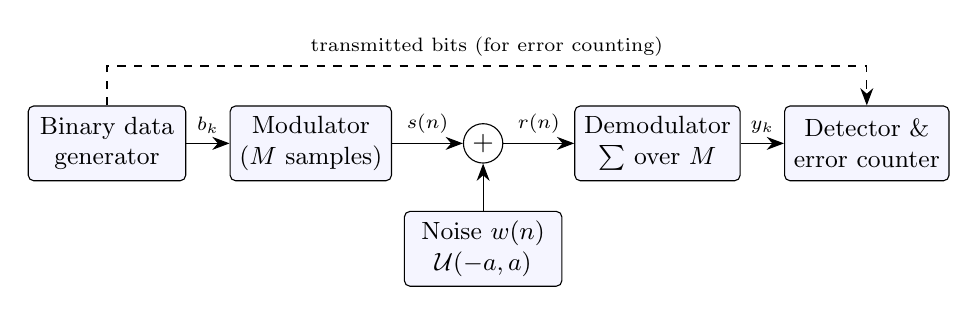
\begin{tikzpicture}[
  blk/.style={draw, rounded corners=2pt, minimum height=0.95cm, minimum width=2.0cm,
              align=center, font=\small, fill=blue!4},
  sum/.style={draw, circle, inner sep=0pt, minimum size=0.5cm},
  >={Stealth[length=2.2mm]}, node distance=0.55cm]
  \node[blk] (src) {Binary data\\generator};
  \node[blk, right=of src] (mod) {Modulator\\($M$ samples)};
  \node[sum, right=0.9cm of mod] (add) {$+$};
  \node[blk, right=0.9cm of add] (dem) {Demodulator\\$\sum$ over $M$};
  \node[blk, right=of dem] (det) {Detector \&\\error counter};
  \node[blk, below=0.6cm of add] (noi) {Noise $w(n)$\\$\mathcal{U}(-a,a)$};
  \draw[->] (src) -- node[above, font=\scriptsize]{$b_k$} (mod);
  \draw[->] (mod) -- node[above, font=\scriptsize]{$s(n)$} (add);
  \draw[->] (add) -- node[above, font=\scriptsize]{$r(n)$} (dem);
  \draw[->] (dem) -- node[above, font=\scriptsize]{$y_k$} (det);
  \draw[->] (noi) -- (add);
  \draw[->, dashed] (src.north) -- ++(0,0.5) -| node[pos=0.25, above, font=\scriptsize]{transmitted bits (for error counting)} (det.north);
\end{tikzpicture}
\caption{Binary data communication system of Project 12.7 (after Fig.~12.16 of~\cite{ingle2017}).}
\label{fig:block127}
\end{figure}

\begin{figure}[t]
\centering
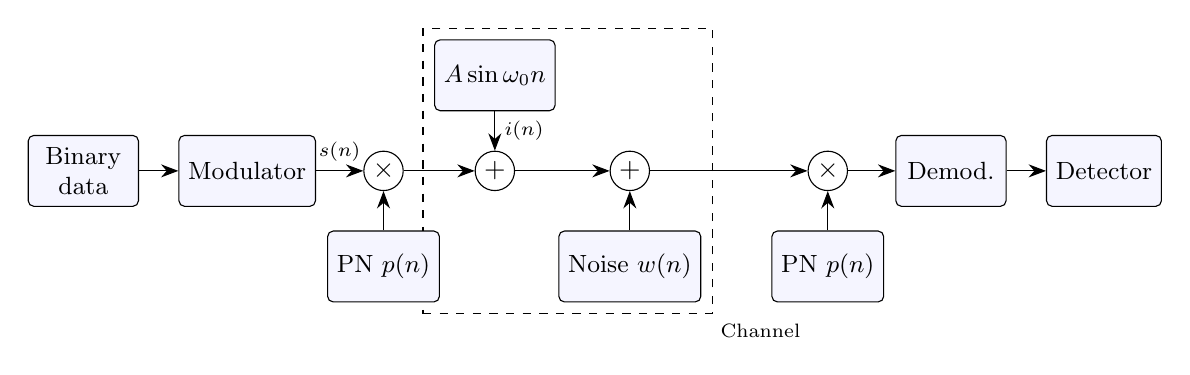
\begin{tikzpicture}[
  blk/.style={draw, rounded corners=2pt, minimum height=0.9cm, minimum width=1.4cm,
              align=center, font=\small, fill=blue!4},
  mul/.style={draw, circle, inner sep=0pt, minimum size=0.5cm},
  >={Stealth[length=2.2mm]}, node distance=0.5cm]
  \node[blk] (src) {Binary\\data};
  \node[blk, right=of src] (mod) {Modulator};
  \node[mul, right=0.6cm of mod] (x1) {$\times$};
  \node[mul, right=0.9cm of x1] (a1) {$+$};
  \node[mul, right=1.2cm of a1] (a2) {$+$};
  \node[mul, right=2.0cm of a2] (x2) {$\times$};
  \node[blk, right=0.6cm of x2] (dem) {Demod.};
  \node[blk, right=of dem] (det) {Detector};
  \node[blk, below=0.5cm of x1] (pn1) {PN $p(n)$};
  \node[blk, above=0.5cm of a1] (sin) {$A\sin\omega_0 n$};
  \node[blk, below=0.5cm of a2] (noi) {Noise $w(n)$};
  \node[blk, below=0.5cm of x2] (pn2) {PN $p(n)$};
  \draw[->] (src) -- (mod);
  \draw[->] (mod) -- node[above, font=\scriptsize]{$s(n)$} (x1);
  \draw[->] (x1) -- (a1);
  \draw[->] (a1) -- (a2);
  \draw[->] (a2) -- (x2);
  \draw[->] (x2) -- (dem);
  \draw[->] (dem) -- (det);
  \draw[->] (pn1) -- (x1);
  \draw[->] (sin) -- node[right, font=\scriptsize]{$i(n)$} (a1);
  \draw[->] (noi) -- (a2);
  \draw[->] (pn2) -- (x2);
  \begin{scope}[on background layer]
    \node[draw, dashed, fit=(sin)(a1)(a2)(noi), inner sep=4pt, label={[font=\scriptsize]below right:Channel}] {};
  \end{scope}
\end{tikzpicture}
\caption{Binary PN spread-spectrum system of Project 12.8 (after Fig.~12.18 of~\cite{ingle2017}).
The same PN sequence is used at the transmitter and the (synchronised) receiver.}
\label{fig:block128}
\end{figure}

% ================================================================ theory
\section{Theory}\label{sec:theory}

\subsection{Binary system with additive noise}

Bit $b_k\in\{0,1\}$ is mapped to the antipodal level $d_k = 2b_k - 1 = \pm1$ and
repeated for $M$ samples,
\begin{equation}
  s(n) = d_k, \qquad kM \le n < (k+1)M .
\end{equation}
The channel adds i.i.d.\ noise $w(n)\sim\mathcal{U}(-a,a)$ with power
$P_n = \mathrm{E}[w^2] = a^2/3$. The demodulator sums the $M$ received samples of
each bit,
\begin{equation}
  y_k = \sum_{n=kM}^{(k+1)M-1} r(n) = M d_k + \underbrace{\sum_{n} w(n)}_{W_k},
  \label{eq:yk}
\end{equation}
which is the matched filter (integrate-and-dump) for a rectangular pulse. The
detector decides $\hat b_k = 1$ if $y_k>0$. The signal component has energy $M^2$
and the noise component $W_k$ has variance $MP_n$, so the post-detection SNR is
$M^2/(MP_n) = M/P_n$, which is the definition used in the brief:
\begin{equation}
  \snr = \frac{M}{P_n}.
\end{equation}
By symmetry the bit error probability is $P_e = \Pr\{W_k > M\}$.

\paragraph{Gaussian approximation.} For large $M$ the central limit theorem gives
$W_k\approx\mathcal{N}(0, MP_n)$ and
\begin{equation}
  P_e \approx \Q\!\left(\frac{M}{\sqrt{MP_n}}\right) = \Q\!\left(\sqrt{\snr}\right),
  \qquad \Q(x)=\tfrac12\operatorname{erfc}(x/\sqrt2).
  \label{eq:pe_gauss}
\end{equation}

\paragraph{Exact result.} $W_k$ is a sum of $M$ independent uniform variables, so
$W_k = 2aS - Ma$ where $S$ is a sum of $M$ independent $\mathcal{U}(0,1)$ variables,
which has the Irwin--Hall distribution. Hence
\begin{equation}
  P_e = \Pr\{S > x\} = F_M(M-x), \qquad x = \frac{M(1+a)}{2a},\qquad
  F_M(y) = \frac{1}{M!}\sum_{k=0}^{\lfloor y\rfloor}(-1)^k\binom{M}{k}(y-k)^M ,
  \label{eq:pe_exact}
\end{equation}
using the symmetry of $S$ about $M/2$. Evaluating $F_M$ on the short side
($y\le M/2$) keeps the alternating sum well conditioned; for the $M\le20$ used here
the double-precision values agree with a 50-digit evaluation to at least seven
significant figures (\texttt{exact\_ber\_uniform.m}). Two special cases are useful
checks: for $M=1$, $P_e = (a-1)/(2a)$ for $a>1$; and for any $M$, $P_e = 0$ when
$a\le1$ because $|W_k|\le Ma \le M$. Because the true density has bounded support,
its tails fall off faster than the Gaussian, so \eqref{eq:pe_gauss} overestimates
$P_e$ at high SNR.

\subsection{Sinusoidal jamming without spreading}

With the jammer present, $y_k = Md_k + W_k + J_k$, where
\begin{equation}
  J_k = A\sum_{n=kM}^{kM+M-1}\sin\omega_0 n
      = A\,\underbrace{\frac{\sin(M\omega_0/2)}{\sin(\omega_0/2)}}_{D_M(\omega_0)}
        \sin\!\Big(\omega_0\big(kM + \tfrac{M-1}{2}\big)\Big).
  \label{eq:jk}
\end{equation}
$D_M$ is the Dirichlet kernel: the integrate-and-dump demodulator is a low-pass
filter with gain $M$ at DC, main lobe $|\omega_0|<2\pi/M$ and nulls at
$\omega_0 = 2\pi\ell/M$. Two regimes follow.
\begin{itemize}
  \item \textbf{In-band jammer} ($\omega_0 \ll 2\pi/M$): $D_M\approx M$, so the
        jammer is integrated exactly like the signal, $|J_k|$ reaches $AM$, and an
        error occurs whenever $|A\sin(\cdot)|>1$. Increasing $M$ does \emph{not} help.
  \item \textbf{Out-of-band jammer}: $|J_k|\le A/|\sin(\omega_0/2)|$, independent of
        $M$, so the demodulator already rejects it unless $A$ is very large.
\end{itemize}
Averaging over the jammer phase $\phi$ at the start of a bit (uniform for
incommensurate $\omega_0$) and treating $W_k$ as Gaussian,
\begin{equation}
  P_e^{\text{no PN}} = \mathrm{E}_\phi\!\left[\tfrac12\Q\!\left(\frac{M+J(\phi)}{\sqrt{MP_n}}\right)
     + \tfrac12\Q\!\left(\frac{M-J(\phi)}{\sqrt{MP_n}}\right)\right].
  \label{eq:pe_nopn}
\end{equation}

\subsection{Direct-sequence spreading}

The transmitter sends $s(n)p(n)$, where $p(n)=\pm1$ are equiprobable i.i.d.\ chips.
The receiver multiplies by the same $p(n)$; since $p^2(n)=1$,
\begin{equation}
  r(n)p(n) = s(n) + w(n)p(n) + A\sin(\omega_0 n)\,p(n).
\end{equation}
The desired signal is restored exactly, the noise is statistically unchanged, and
the jammer is multiplied by a random $\pm1$ sequence. Its spectrum is therefore
spread uniformly over $(-\pi,\pi]$: the jammer becomes zero-mean white noise of
power $A^2/2$. After summing over a bit,
\begin{equation}
  J_k' = A\sum_n p(n)\sin\omega_0 n,\qquad
  \mathrm{E}[J_k']=0,\qquad \operatorname{Var}[J_k'] = A^2\sum_n\sin^2\omega_0 n \approx \frac{MA^2}{2},
\end{equation}
and the signal-to-interference-plus-noise ratio at the detector is
\begin{equation}
  \mathrm{SINR} = \frac{M^2}{MP_n + MA^2/2} = \frac{M}{P_n + A^2/2},
  \qquad P_e^{\text{PN}} \approx \Q\!\left(\sqrt{\frac{M}{P_n + A^2/2}}\right).
  \label{eq:pe_pn}
\end{equation}
Comparing with the per-sample signal-to-jammer ratio $2/A^2$ shows a
\emph{processing gain} $G_p = M$ ($10\log_{10}M$ dB): spreading lets the
integrator average the jammer down in exactly the way it averages white noise.
For very low $\omega_0$ the factor $\sum\sin^2$ differs from bit to bit, so the
simulations are compared with the phase-averaged form
$\mathrm{E}_\phi\big[\Q\big(M/\sqrt{MP_n + A^2\sum\sin^2(\omega_0n+\phi)}\big)\big]$
(\texttt{ber\_theory\_jam.m}).

\paragraph{Consequence for the condition $A\ge M$.} The jammer-to-signal power ratio
is $\mathrm{JSR}=A^2/2$, so with $A=M$ it is $M^2/2$ while the processing gain is
only $M$. \Cref{eq:pe_pn} then gives $\mathrm{SINR}\approx2/M$, which
\emph{decreases} with $M$: under the brief's condition neither system can reach a
low error rate, and the comparison must be read in terms of which system degrades
less. This prediction is confirmed in \cref{sec:res128}.

% ================================================================ implementation
\section{MATLAB implementation}\label{sec:impl}

\subsection{Structure}

Each block of \cref{fig:block127,fig:block128} is a separate function in the
\texttt{matlab/} folder (\cref{tab:functions}); the five functions required by
Project 12.7 are reused unchanged in Project 12.8. The code uses only core MATLAB
(no toolboxes) and also runs in GNU Octave, which was used to produce the
results in this report. Full listings are in \cref{app:code}.

\begin{table}[ht]
\centering
\caption{MATLAB functions and the block each implements.}
\label{tab:functions}
\begin{tabular}{@{}lll@{}}
\toprule
Function & Block & Operation \\
\midrule
\texttt{bit\_generator(N)}          & Binary data generator & $b_k = [u_k\ge0.5]$, $u_k\sim\mathcal{U}(0,1)$ \\
\texttt{modulator(b,M)}             & Modulator             & repeat $2b_k-1$ for $M$ samples \\
\texttt{noise\_generator(L,a)}      & Noise generator       & $a(2u-1)$, uniform on $(-a,a)$ \\
\texttt{demodulator(r,M)}           & Demodulator           & column sums of an $M\times N$ reshape \\
\texttt{detector(y,b)}              & Detector \& counter   & $\hat b_k=[y_k>0]$, count $\hat b_k\ne b_k$ \\
\texttt{pn\_generator(L)}           & PN generator          & equiprobable $\pm1$ chips \\
\texttt{sine\_generator(L,A,w0,n0)} & Sine generator        & $A\sin\omega_0 n$, continuous phase \\
\midrule
\texttt{binary\_comm\_sim}          & Whole system          & chains the blocks, Monte-Carlo loop \\
\texttt{exact\_ber\_uniform}        & Theory                & exact $P_e$, Irwin--Hall \eqref{eq:pe_exact} \\
\texttt{ber\_theory\_jam}           & Theory                & \cref{eq:pe_nopn,eq:pe_pn}, phase averaged \\
\bottomrule
\end{tabular}
\end{table}

The core of the simulator, \texttt{binary\_comm\_sim}, follows the block diagram
line by line:
\begin{lstlisting}[firstnumber=29]
b  = bit_generator(Nb);                 % binary data generator
s  = modulator(b, M);                   % modulator
if use_pn
    p = pn_generator(L);                % PN sequence generator
    s = s .* p;                         % spreading
end
r = s + noise_generator(L, a);          % channel: wideband noise
if A ~= 0
    r = r + sine_generator(L, A, w0, n0);   % channel: sine jammer
end
if use_pn
    r = r .* p;                         % despreading
end
y = demodulator(r, M);                  % demodulator
[~, e] = detector(y, b);                % detector / error counter
\end{lstlisting}

\subsection{Simulation design}

\begin{itemize}
  \item \textbf{Vectorisation and memory.} Bits are processed in blocks of up to
        $2\times10^7$ samples so that $M=1000$ runs do not exhaust memory; the
        jammer sample index $n_0$ is carried between blocks so its phase is continuous.
  \item \textbf{Stopping rule.} For Project 12.7 each SNR point runs until 200 errors
        are counted or $2\times10^7$ bits are simulated. With 200 errors the relative
        standard error of the BER estimate is about $1/\sqrt{200}\approx7\%$.
        For the $A=M$ experiment a fixed budget of $2\times10^7$ samples per point
        ($4\times10^5$ bits at $M=50$, $2\times10^4$ bits at $M=1000$) was used;
        at BER $\approx0.45$ this gives a standard error below $0.004$.
  \item \textbf{Parameters.} Unless stated otherwise $P_n=1$ ($a=\sqrt3$). Two jammer
        frequencies were used: $\omega_0=0.002$~rad/sample, inside the demodulator
        pass-band $2\pi/M$ for every $M$ tested, and $\omega_0=1$~rad/sample
        ($\approx0.318\pi$), outside it. Both are deliberately incommensurate with
        $2\pi/M$; a frequency such as $0.1\pi$ with $M=100$ places the jammer exactly
        on a null of $D_M$ and gives a misleading zero error rate.
  \item \textbf{Reproducibility.} Seeds are fixed with \texttt{rng}; \texttt{run\_all.m}
        regenerates every number and figure, and the tables in this report are read
        directly from the files the scripts write.
\end{itemize}

% ================================================================ results 12.7
\section{Results: Project 12.7}\label{sec:res127}

\Cref{fig:wave} traces eight bits through the system at $M=10$, $P_n=1$
($\snr=\SI{10}{dB}$). The received samples are individually unreliable (many have
the wrong sign), but summing $M$ of them gives decision statistics close to
$\pm10$ and all eight bits are detected correctly.

\begin{figure}[ht]
\centering
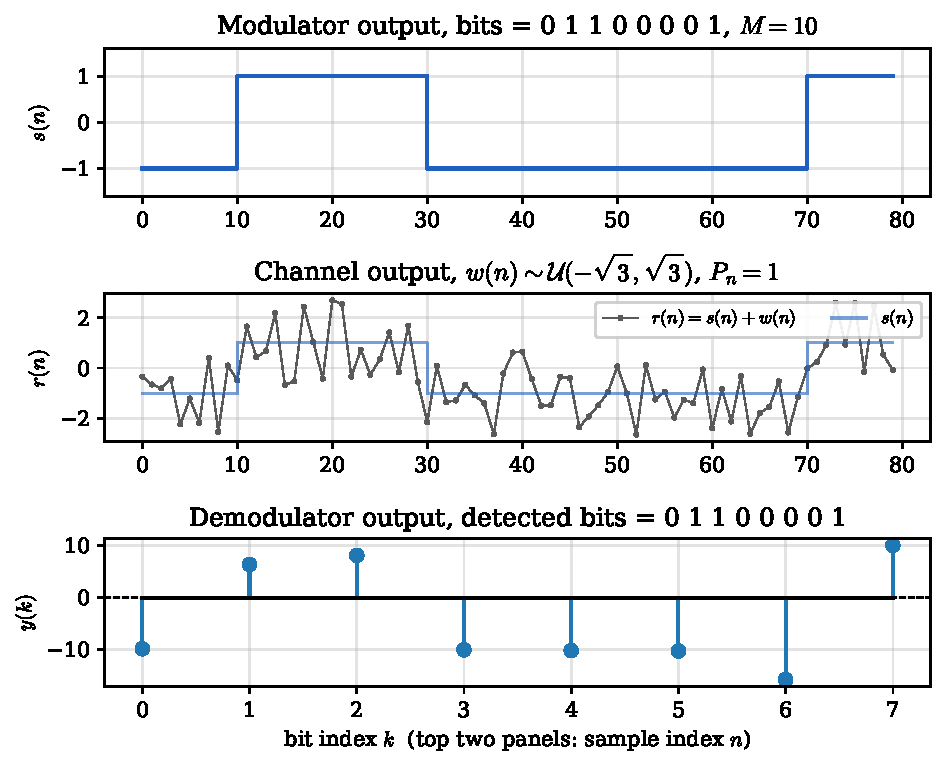
\includegraphics[width=0.82\linewidth]{p127_waveforms}
\caption{Signals at the modulator output, channel output and demodulator output for
$M=10$ and $P_n=1$.}
\label{fig:wave}
\end{figure}

The BER was measured in the two ways suggested in the brief: (a) $P_n=1$ fixed with
$M=1,\dots,20$, and (b) $M=10$ fixed with $P_n$ varied to give
$\snr=0$--$\SI{13}{dB}$. \Cref{fig:ber127} and \cref{tab:127} show the results.

\begin{figure}[ht]
\centering
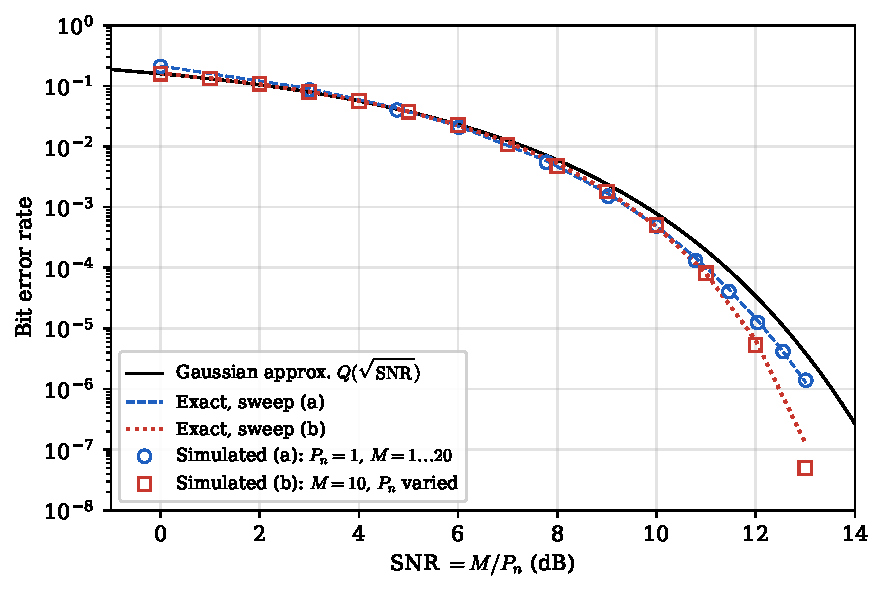
\includegraphics[width=0.78\linewidth]{p127_ber}
\caption{BER against $\snr=M/P_n$ for the binary system with uniform noise.}
\label{fig:ber127}
\end{figure}

\begin{table}[ht]
\centering
\caption{Sweep (a): $P_n=1$, $M$ varied. Simulated BER compared with the exact
probability and the Gaussian approximation $\Q(\sqrt{\snr})$.}
\label{tab:127}
\small
\begin{tabular}{@{}rrcccr@{}}
\toprule
$M$ & SNR (dB) & Simulated & Exact & $\Q(\sqrt{\snr})$ & Bits \\
\midrule
\inputrows{../results/table_127.tex}
\bottomrule
\end{tabular}
\end{table}

Observations:
\begin{enumerate}
  \item The BER falls steeply with SNR, from about $0.2$ at \SI{0}{dB} to
        $10^{-6}$ near \SI{13}{dB}; each extra dB costs roughly a factor of three
        to ten in BER at high SNR.
  \item The simulation agrees with the exact result at every point within the
        expected Monte-Carlo scatter, which validates the implementation of all five
        blocks. At $M=1$ the simulated $0.21$ matches $(a-1)/(2a)=0.211$.
  \item The Gaussian approximation is accurate between about 3 and \SI{8}{dB} but
        is optimistic at $M=1$ (a single uniform sample has heavier mass near its
        edges than a Gaussian) and increasingly pessimistic at high SNR, by a factor
        of three at \SI{13}{dB} in sweep (a).
  \item The two sweeps coincide at low SNR, as the definition $\snr=M/P_n$ implies,
        but separate at high SNR: for sweep (b) with $M=10$ fixed, high SNR means a
        small noise range $a$, and as $a\to1$ the maximum possible noise sum $Ma$
        approaches $M$, so $P_e\to0$ much faster than the Gaussian tail. Only
        one error in $2\times10^7$ bits was observed at \SI{13}{dB}, consistent with
        the exact value $1.2\times10^{-7}$. The SNR alone does not fully describe the
        system when the noise is not Gaussian.
\end{enumerate}

% ================================================================ results 12.8
\section{Results: Project 12.8}\label{sec:res128}

\subsection{The brief's experiment: \texorpdfstring{$A=M$}{A = M}}

\Cref{tab:128} and \cref{fig:aeqm} give the BER with and without the PN sequence for
$M=50,100,500,1000$ with the smallest jammer amplitude the brief allows, $A=M$.

\begin{table}[ht]
\centering
\caption{BER with the jammer amplitude $A=M$ and $P_n=1$. Each entry is
\emph{simulated (theory)}, with theory from the phase-averaged
\cref{eq:pe_nopn,eq:pe_pn} (Gaussian approximation for the summed noise).}
\label{tab:128}
\small
\begin{tabular}{@{}rr cc cc@{}}
\toprule
 & & \multicolumn{2}{c}{In-band, $\omega_0=0.002$} & \multicolumn{2}{c}{Out-of-band, $\omega_0=1$} \\
\cmidrule(lr){3-4}\cmidrule(l){5-6}
$M$ & $A$ & No PN & PN & No PN & PN \\
\midrule
\inputrows{../results/table_128.tex}
\bottomrule
\end{tabular}
\end{table}

\begin{figure}[ht]
\centering
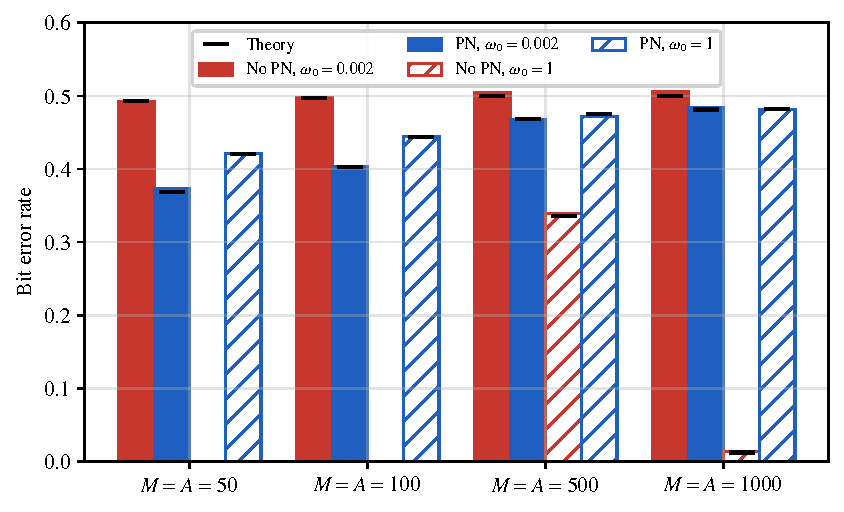
\includegraphics[width=0.78\linewidth]{p128_ber_A_eq_M}
\caption{BER at $A=M$; black ticks mark the theoretical values.}
\label{fig:aeqm}
\end{figure}

\begin{itemize}
  \item \textbf{In-band jammer.} Without PN the BER is $0.49$--$0.50$ for every $M$:
        the jammer passes through the integrator with the full gain $M$, so the bit
        sum is dominated by $AM\sin(\cdot)$ and the decision is essentially a coin
        toss. With PN the BER is lower, $0.37$ at $M=50$, because the jammer has been
        converted into noise whose bit-sum standard deviation is only
        $A\sqrt{M/2}$. The improvement shrinks as $M$ grows because
        $\mathrm{SINR}\approx 2/M$ when $A=M$.
  \item \textbf{Out-of-band jammer.} Without PN the demodulator rejects the jammer
        through its $\sin(\omega_0/2)$ roll-off. What matters is the peak jammer sum
        $A|D_M(1)|$ relative to the signal sum $M$; with $A=M$ this ratio is
        $|D_M(1)| = 0.28$, $0.55$, $2.02$ and $0.98$ for $M=50$, $100$, $500$ and
        $1000$. For $M=50$ and $100$ the jammer can never overturn a bit and the BER is
        $0$. For $M=500$ it overturns every bit whose jammer phase is near the peak,
        giving BER $=0.33$. For $M=1000$ the ratio is just below 1, so the jammer alone
        cannot cause an error; the residual BER of $0.013$ comes from the noise
        (standard deviation $\sqrt{MP_n}=32$) pushing bits that the jammer has brought
        within $0.02M=20$ of the threshold across it. With PN the BER is $0.42$--$0.48$
        at both jammer frequencies and is therefore \emph{worse} here: spreading takes
        a jammer the receiver was already rejecting and turns it into in-band noise.
  \item The simulated and theoretical values agree to within $\pm0.007$ in every
        cell, so the behaviour is a property of the system, not of the simulation.
\end{itemize}

\subsection{Effect of jammer power}

To see the processing gain directly, the in-band jammer amplitude was swept from
$A=0.1$ to $1000$ (\cref{fig:jsr}), and the jammer-to-signal ratio at which each
system reaches BER $=10^{-3}$ was read from the theory curves (\cref{tab:margin}).

\begin{figure}[ht]
\centering
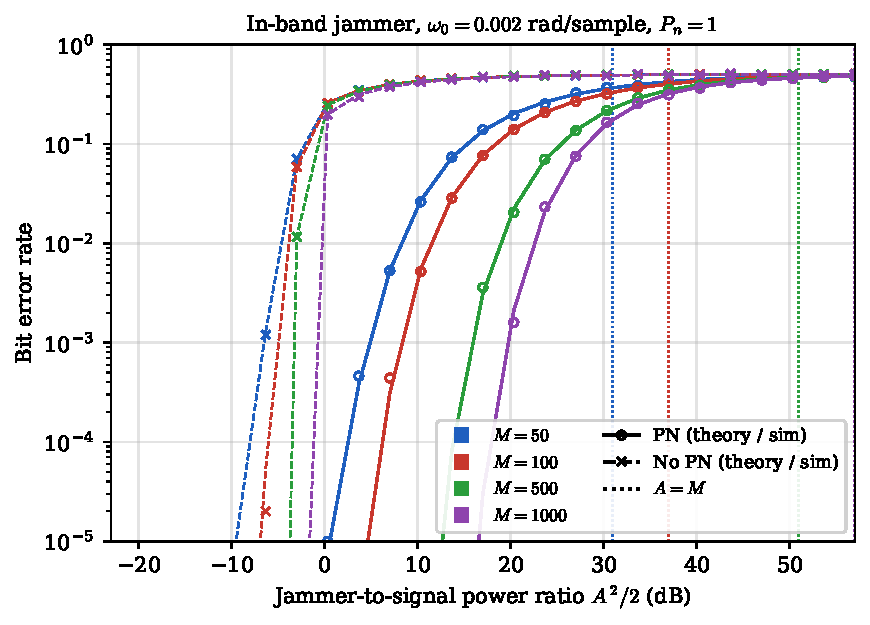
\includegraphics[width=0.8\linewidth]{p128_ber_vs_jsr}
\caption{BER against jammer-to-signal power ratio $A^2/2$ for the in-band jammer.
Solid lines and circles: PN; dashed lines and crosses: no PN. Dotted verticals mark
$A=M$ for each $M$.}
\label{fig:jsr}
\end{figure}

\begin{table}[ht]
\centering
\caption{Jammer-to-signal ratio (dB) tolerated at BER $=10^{-3}$, in-band jammer,
$P_n=1$, and the ratio implied by the brief's condition $A=M$.}
\label{tab:margin}
\small
\begin{tabular}{@{}rccccc@{}}
\toprule
$M$ & $10\log_{10}M$ & No PN & PN & Improvement & JSR at $A=M$ \\
\midrule
\inputrows{../results/table_margin.tex}
\bottomrule
\end{tabular}
\end{table}

Without PN every curve breaks at roughly the same point, $\mathrm{JSR}\approx-3$
to \SI{0}{dB}, i.e.\ $A\approx1$: once the jammer amplitude exceeds the signal
amplitude, errors occur no matter how many samples are integrated. With PN the
curves move right by roughly $10\log_{10}M$, and the improvement in
\cref{tab:margin} grows from \SI{11}{dB} at $M=50$ to \SI{20}{dB} at $M=1000$.
The improvement is below the ideal $10\log_{10}M$ because a jammer this slow does
not average its $\sin^2$ within one bit, so some bits see more interference than
others, and because the noise still contributes. The last column shows why the
$A=M$ experiment saturates: the jammer is \SIrange{26}{37}{dB} stronger than the
PN system can tolerate.

\subsection{Effect of jammer frequency}

\Cref{fig:w0} sweeps $\omega_0$ over $0.002\pi\le\omega_0\le0.998\pi$ for $M=100$;
the end points are excluded because the brief requires $0<\omega_0<\pi$, and at
$\omega_0=\pi$ the sampled jammer $A\sin(\pi n)$ is identically zero. With PN the
BER is nearly constant over most of the band and agrees with \cref{eq:pe_pn}:
$0.44$ at $A=100$, and $\Q(\sqrt{100/13.5})=3.2\times10^{-3}$ at $A=5$. It rises
within roughly $2\pi/M$ of either band edge, where $\sin^2\omega_0 n$ is no longer
averaged within one bit, so the despread interference power varies from bit to bit;
the phase-averaged theory reproduces this. Without PN the BER follows
the Dirichlet kernel $|D_M(\omega_0)|$: it is $0.5$ near DC, falls to zero at every
null $\omega_0=2\pi\ell/M$, and decays with $\omega_0$. At $A=5$ the system without
PN fails only for $\omega_0<0.03\pi$, i.e.\ inside the main lobe of the
demodulator response.

\begin{figure}[ht]
\centering
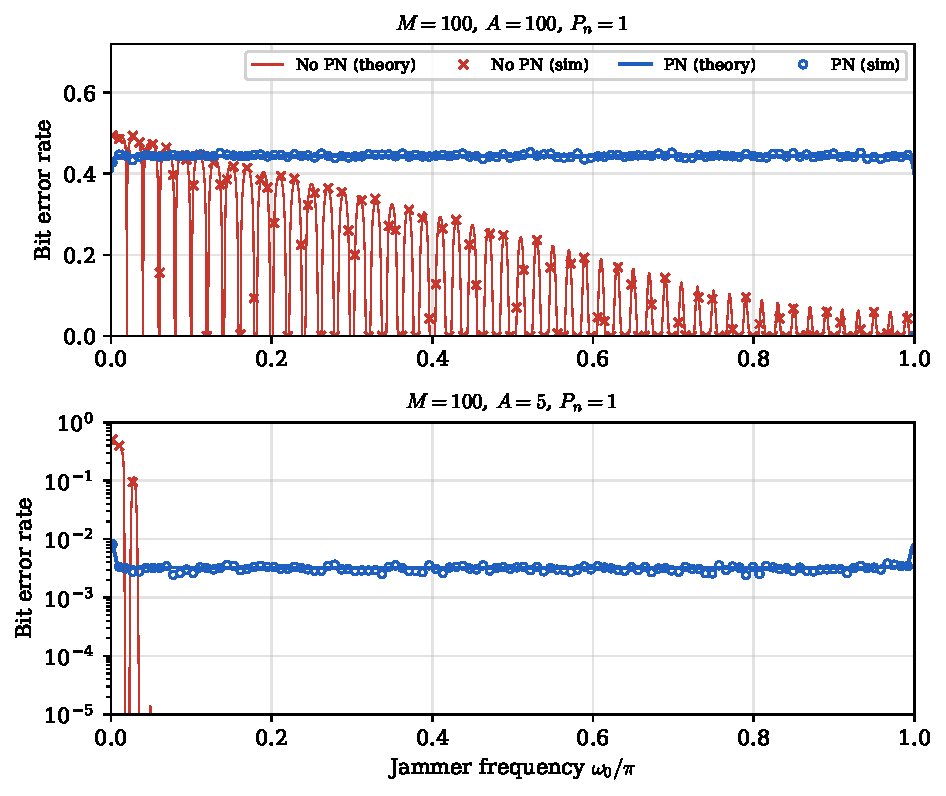
\includegraphics[width=0.8\linewidth]{p128_ber_vs_w0}
\caption{BER against jammer frequency for $M=100$ and $0<\omega_0<\pi$: $A=M$ (top,
linear scale) and $A=5$ (bottom, log scale). Theory curves are the phase-averaged
expressions of \cref{sec:theory}.}
\label{fig:w0}
\end{figure}

\subsection{Spectral view}

\Cref{fig:psd} shows the power spectral densities before and after despreading for
$M=100$, $A=10$, $\omega_0=0.2\pi$. In the channel the spread signal is white with
power 1 (\SI{0}{dB}), as is the noise, while the jammer is a line \SI{40}{dB}
above them. After despreading the roles swap: the desired signal collapses back into
the narrow $\mathrm{sinc}^2$ spectrum of a rectangular pulse, with \SI{20}{dB}
($=10\log_{10}M$) at DC, and the jammer becomes a white floor at
$10\log_{10}(A^2/2)=\SI{17}{dB}$. The integrate-and-dump demodulator passes only
the band $|\omega|\lesssim2\pi/M$, which contains all of the signal energy but only
a fraction of order $1/M$ of the spread jammer power.

\begin{figure}[ht]
\centering
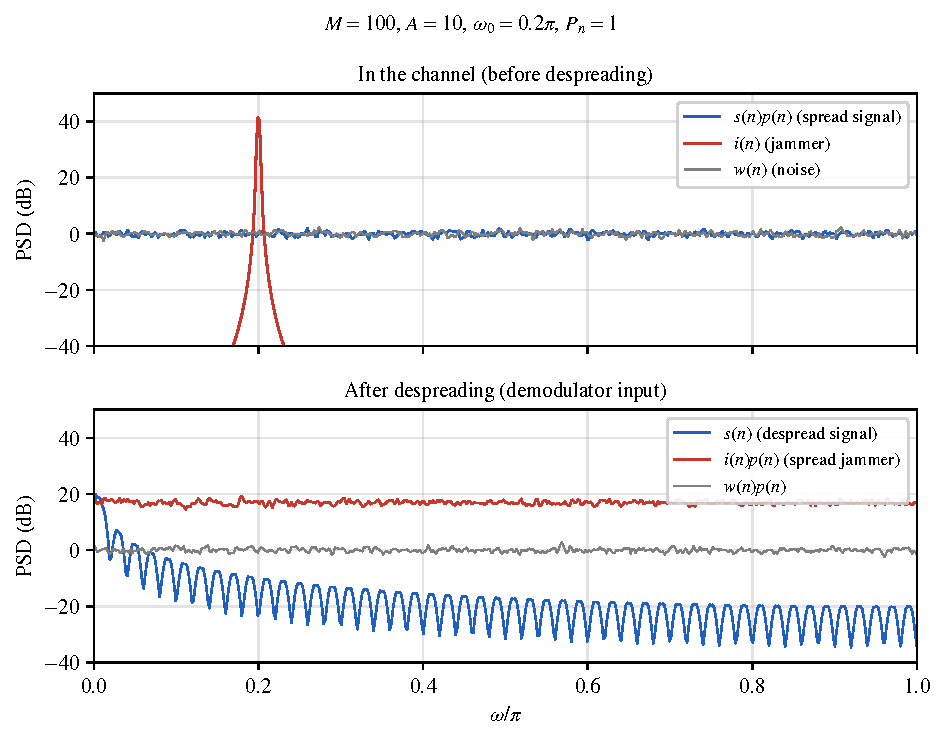
\includegraphics[width=0.8\linewidth]{p128_spectra}
\caption{Power spectral densities (Hann-windowed averaged periodogram) in the channel
and after despreading.}
\label{fig:psd}
\end{figure}

% ================================================================ discussion
\section{Discussion}\label{sec:discussion}

\subsection{Effect of the PN sequence on the sinusoidal interference}

Multiplying by a random $\pm1$ sequence is a modulation by a wideband signal. In the
frequency domain the jammer spectrum, a pair of lines at $\pm\omega_0$, is convolved
with the flat spectrum of $p(n)$, so the receiver's despreading multiplier turns the
sinusoid into white noise of the same power $A^2/2$ (\cref{fig:psd}). The same
operation applied to the desired signal, which was spread by the same $p(n)$, undoes
the spreading because $p^2(n)=1$. The PN sequence therefore acts as a key that
concentrates only the signal back into the narrow band of the demodulator.

\subsection{Why the spread-spectrum system outperforms the conventional one}

\begin{enumerate}
  \item \textbf{Processing gain.} The demodulator sums $M$ samples. The desired signal
        adds coherently (amplitude $M$, power $M^2$), but the despread jammer adds
        incoherently (power $MA^2/2$), giving a gain of $M$ in signal-to-jammer ratio.
        Without PN, an in-band jammer adds coherently as well, so integration gives no
        gain at all; this is why the conventional system fails at $A\approx1$ whatever
        $M$ is, while the PN system tolerates jammers \SIrange{11}{20}{dB} stronger
        (\cref{tab:margin}).
  \item \textbf{Weak dependence on the jammer frequency.} Away from the band edges
        (within about $2\pi/M$ of $\omega_0=0$ or $\pi$) the PN system's performance
        depends essentially on the jammer power alone (\cref{fig:w0}). A jammer
        cannot find a frequency where the receiver is much weaker; its best strategy is
        simply more power. In the conventional system the worst case, a jammer placed
        inside the signal band, is also the easiest for an adversary to choose.
  \item \textbf{Low probability of interception.} Although not measured here, the
        spread signal has a flat spectrum at the noise level (\cref{fig:psd}), which
        makes it difficult to detect or to target, and different PN codes allow
        several users to share the band (CDMA).
\end{enumerate}

\subsection{Interpreting the condition \texorpdfstring{$A\ge M$}{A >= M}}

The brief asks for $A\ge M$. As derived in \cref{sec:theory} and confirmed by
\cref{tab:128}, this places the jammer \SIrange{31}{57}{dB} above the signal, beyond
the $10\log_{10}M=\SIrange{17}{30}{dB}$ processing gain, so neither system works
reliably and the PN system's advantage appears only as a lower error rate against an
in-band jammer ($0.37$ against $0.49$ at $M=50$). We also found that for an
out-of-band jammer the conventional system can be better, because its integrator
already rejects the tone. Rather than suggesting that spread spectrum is ineffective,
this shows that the benefit is a fixed number of decibels: to obtain a low error
rate with $A=M$ the processing gain would need to grow as $M^2$, which this system's
single-PN-chip-per-sample structure cannot provide. Practical systems such as GPS
obtain their \SI{43}{dB} processing gain from a chip rate $2\times10^4$ times the
bit rate.

\subsection{Limitations}

\begin{itemize}
  \item Perfect bit and code synchronisation was assumed; in practice code
        acquisition and tracking are a significant part of a DSSS receiver.
  \item The PN sequence is generated by a random number generator, as the brief
        allows. Real systems use deterministic maximal-length or Gold sequences, whose
        autocorrelation and cross-correlation properties are guaranteed.
  \item Uniform noise was used as specified; a thermal-noise channel would be
        Gaussian, for which \cref{eq:pe_gauss} is exact.
  \item The Gaussian treatment of the despread jammer in \cref{eq:pe_pn} is
        accurate for large $M$; at $M=50$ the simulation and theory still agree
        within $0.007$.
\end{itemize}

% ================================================================ conclusion
\section{Conclusion}

Both textbook systems were implemented in MATLAB as one function per block and
validated against analytical results. For the binary system with uniform noise the
BER follows the exact Irwin--Hall result over seven decades, and the
familiar $\Q(\sqrt{\snr})$ approximation is pessimistic at high SNR because the
noise is bounded. For the spread-spectrum system, the PN sequence converts a
narrowband jammer into wideband noise, which the integrate-and-dump demodulator then
averages down by the processing gain $M$. This made the receiver tolerate in-band
jammers \SIrange{11}{20}{dB} stronger than the conventional receiver and made its
performance nearly independent of the jammer frequency away from the band edges. Under the brief's condition $A=M$
the jammer power exceeds the processing gain by \SIrange{14}{27}{dB}, so both systems
operate near BER $=0.5$; the PN system still has the lower error rate against an
in-band jammer, but not against an out-of-band one, which the conventional
demodulator already filters out.

% ================================================================ contribution
\section*{Individual contribution}
\addcontentsline{toc}{section}{Individual contribution}
[Describe your own contribution to the group work here: for example which blocks you
implemented, which experiments you ran, and which parts of the analysis you led.]

% ================================================================ references
\begin{thebibliography}{9}
\bibitem{ingle2017} V.~K.~Ingle and J.~G.~Proakis, \emph{Digital Signal Processing
  Using MATLAB}, 4th~ed. Boston, MA: Cengage Learning, 2017, Projects 12.7 and 12.8.
\bibitem{proakis2008} J.~G.~Proakis and M.~Salehi, \emph{Digital Communications},
  5th~ed. New York: McGraw-Hill, 2008, ch.~12 (spread-spectrum signals).
\bibitem{sklar2001} B.~Sklar, \emph{Digital Communications: Fundamentals and
  Applications}, 2nd~ed. Upper Saddle River, NJ: Prentice Hall, 2001, ch.~12.
\bibitem{gps} U.S.~Space Force, \emph{Interface Specification IS-GPS-200}, NAVSTAR
  GPS Space Segment/Navigation User Segment Interfaces.
\end{thebibliography}

% ================================================================ appendix
\appendix
\section{MATLAB code}\label{app:code}

\subsection*{Block functions}
\lstinputlisting[caption={bit\_generator.m}]{../matlab/bit_generator.m}
\lstinputlisting[caption={modulator.m}]{../matlab/modulator.m}
\lstinputlisting[caption={noise\_generator.m}]{../matlab/noise_generator.m}
\lstinputlisting[caption={demodulator.m}]{../matlab/demodulator.m}
\lstinputlisting[caption={detector.m}]{../matlab/detector.m}
\lstinputlisting[caption={pn\_generator.m}]{../matlab/pn_generator.m}
\lstinputlisting[caption={sine\_generator.m}]{../matlab/sine_generator.m}

\subsection*{System simulator and theory}
\lstinputlisting[caption={binary\_comm\_sim.m}]{../matlab/binary_comm_sim.m}
\lstinputlisting[caption={exact\_ber\_uniform.m}]{../matlab/exact_ber_uniform.m}
\lstinputlisting[caption={ber\_theory\_jam.m}]{../matlab/ber_theory_jam.m}

\subsection*{Experiment scripts}
\lstinputlisting[caption={project12\_7.m}]{../matlab/project12_7.m}
\lstinputlisting[caption={project12\_8.m}]{../matlab/project12_8.m}

\end{document}
